\documentclass[12pt]{texmemo} % originally by Rob Oakes; adapted by Alice Chen and now Jacob Child
\usepackage{graphicx}
\graphicspath{ {./images/} }
\usepackage{amsmath}
\usepackage{subfigure}

\memoto{ Adam Cardoza, Graduate Student in the BYU FLOW Lab}

\memofrom{Jacob Child}

\memore{Findings from the DJI II Trade Study}

\memodate{\today} % or \today

\memosection{497R (Andrew Ning)}

\begin{document}

\maketitle

\highlight

A set of custom code heavily utilizing the CCBlade.jl package was created in order to analyze variations on the DJI II propeller (A drone propeller made by DJI) The propeller was imported, analyzed, and its geometric and flow properties indecently varied to see the trade-offs and effects on performance. The results and findings are presented below, with a focus on a discussion of the design space rather than the best/optimized parameters.

\textit{When and why do I limit things and how do the parameters influence the design space!}

\textbf{Section I} Discussion of the results that came from varying the blade radius from 5cm to 25cm

\textbf{Section II} Discussion of the results that came from varying the blade pitch from -10 to 20 deg

\textbf{Section III} Discussion of the results that came from varying the blade chord from decreased by 7.5\% to increased 7.5\%

\textbf{Section IV} Discussion of the results that came from varying the Advance Ratio the blades experienced (ie changing vertical speed)

Inside of each section the following items are discussed:

\setlength{\parskip}{0pt} % no new line in list

\begin{itemize}
    \item Coefficient of Thrust trends
    \item Coefficient of power and Torque trends
    \item Figure of Merit Trends
    \item Overall Discussion
\end{itemize}

\setlength{\parskip}{0.5\baselineskip plus 2pt} % reset

\textbf{Section V} concludes this memo with the a very general discussion of the design space with recommendations and limitations of the varied parameters.

\textbf{Appendix} Following the 4 main sections is an appendix containing:

\setlength{\parskip}{0pt} % no new line in list

\begin{itemize}
    \item Surface Plots (not discussed or formatted in favor of brevity and time)
    \item Github overview and high level code explanation
    %\item Extra plots and figures (not discussed in favor of brevity)
\end{itemize}
\newpage 

%%%%%
\section{Findings from varying the blade radius}

The purpose of this section is share the findings from varying the blade radius and how it affects aerodynamic coefficients and their implications on blade performance. 
\vspace{5mm} %5mm vertical space

\begin{figure}[h]
\centering
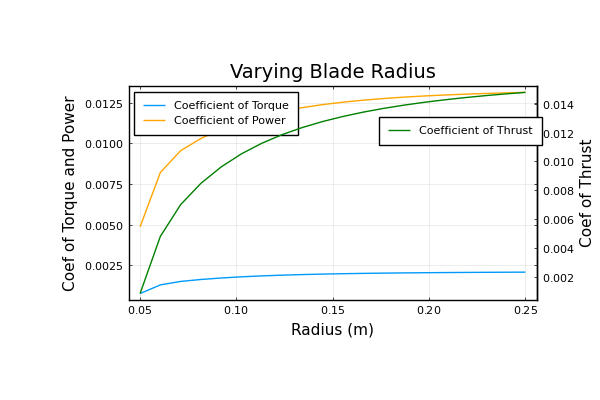
\includegraphics[scale = .75]{RVarCoefHMode.jpg}
\caption{The plot of the change in the coefficients of thrust (right y axis) and torque (left y axis) as the blade radius was increased. There are variances in both the torque and the thrust plots but they are within a minuscule percentage.}
\end{figure}

\textit{Coefficient of Thrust}
$$ C_T = \frac {T}{\rho n^2 R^4} $$
The coefficient of thrust is the amount of thrust the rotor produces normalized with respect to the rpm. CT is relatively flat with only slight up and down movement (it varies less than a tenth of a percent) as the blade radius was varied (See Figure 1). This does not mean that the thrust produced by the blade did not change with the radius, but that the thrust produced increased at almost the same rate as the bottom part of the CT equation $\rho n^2 R^4$, and thus the line is nearly "flat". Knowing the bottom of the CT equation and that both the rpm (n) and air density were kept constant($\rho$) it is found that CT increases at a rate proportional to $R^4$. This is quite a steep increase and shows that lengthening the blade radius is an effective way to increase the amount of thrust a propeller produces. However, the amount of torque and power required to generate that thrust also increases.
\vspace{5mm} %5mm vertical space

\textit{Coefficients of Power and Torque} 
\begin{align}
 C_Q = \frac {Q}{\rho n^2 R^5} 
 \end{align}
Figure 1 shows the plot of the Coefficient of Torque (CQ) and not the Coefficient of Power (CP). This is because CQ and CP can be discussed together and interchangeably as CP is simply $2\pi*CQ$, ie just CQ scaled. At a quick glance it can be seen that CQ is nearly "flat" (See Figure 1). While this is true, it is similar to CT in that torque is simply increasing at the same rate as the bottom of the CQ coefficient equation $\rho n^2 R^5$. This helps to show that although the CT and CQ lines are both "flat" they are not actually increasing at the same rate. CQ increases at a rate proportional to $R^5$ while CT only increases at a rate of $R^4$ which means that CQ, and thus CP also, is increasing quicker than CT when the blade radius increases. This demonstrates that while increasing blade radius is an effective way to increase thrust it comes at the cost of increasing the torque and power necessary to a higher degree.
\vspace{5mm} %5mm vertical space

\begin{figure}[h]
\centering
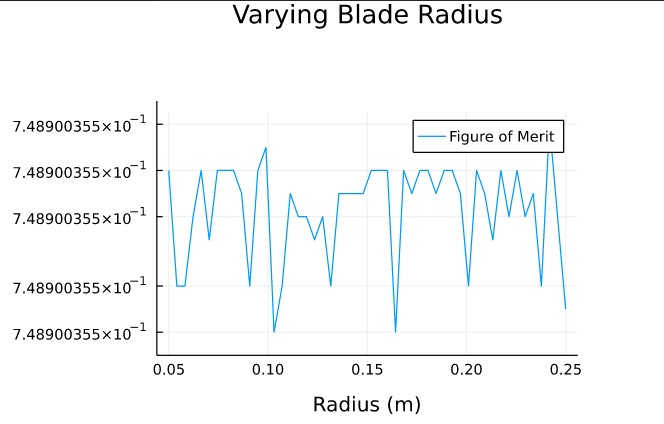
\includegraphics[scale = .75]{RVarFMHmode.jpg}
\caption{The Figure of Merit as it varies with the blade radius.}
\end{figure}
\vspace{5mm} %5mm vertical space

\textit{Figure of Merit} 

\begin{align}
FM = \frac{ C_T^{1.5}}{C_P \sqrt{2}} && FM = \frac{T\sqrt{\frac{T}{2\rho A}}}{P}
\end{align}

The "Figure of Merit" is a way to compare the performance of a helicopter (or drone) propeller as using efficiency doesn't work if the helicopter is simply hovering. It takes the ideal power and divides it by the power actually required as shown on the right side of equation 2. Simplified it becomes the left side of figure 2, the coefficient of thrust to an exponent divided by the coefficient of power scaled by the square root of two. Close inspection of the plot shows that the figure of merit value stays very close to .7489. This is a pretty respectable score and the plot doesn't seem to be increasing in the given range of blade radii. This shows that the power required by this propeller at this rpm is higher than its ideal power draw, but increases at the same rate as the ideal power draw. This means that while increasing the blade radius does increase the amount of thrust it generates, it does not actually change propeller performance with respect to the figure of merit (the score of a small blade radius and a large one are essentially the same). This means that while increasing blade radius is effective, it doesn't "outperform" what would be expected.

\vspace{5mm} %5mm vertical space

%%%%%
\section{Findings from varying the blade pitch}

The purpose of this section is to share the findings from varying the blade pitch and how it affects aerodynamic coefficients and their implications on blade performance. Derivations and explanations discussed above will not be re-discussed for the sake of brevity.

\vspace{5mm} %5mm vertical space

\begin{figure}[h]
\centering
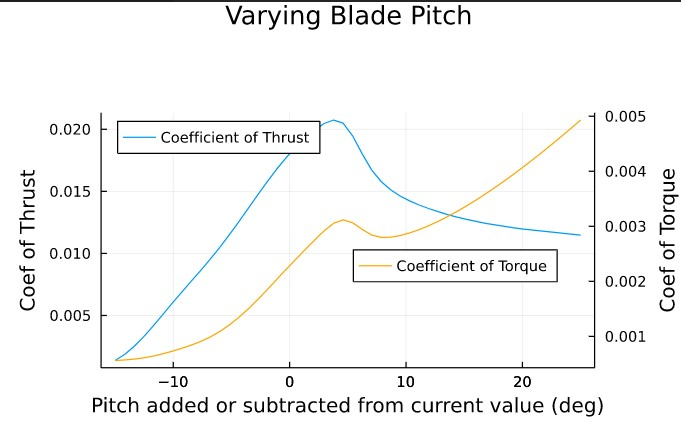
\includegraphics[scale = .75]{PVarCoefHMode.jpg}
\caption{The plot of the change in the coefficients of thrust (left y axis) and torque (right y axis) as the pitch was increased. \textit{Note: The pitch variation was done by adding the shown pitch value to the twist value of each blade section of the standard blade. This means that 0 on the plot is not a horizontal blade, but is the blade in its original orientation as given in the geometry file.}}
\end{figure}

\textit{Coefficient of Thrust}\\
(See equation 1)\\
The Coefficient of Thrust quickly increases as the pitch is increased from a negative to positive orientation. At 0 degrees (what is "normal" for this blade) CT is about .018, but its max happens pitched up by approximately 4 degrees and gives a CT of around .02. This rapid increase shows that changing blade pitch is critical as it can increase or decrease CT at rates that are greater or less than $R^4$ which wasn't the case with varying blade radius. This means that varying the blade pitch is possibly a more effective or "easier" way to increase thrust than varying radius as smaller changes can yield greater results (especially when comparing pitching a blade up vs making a whole new blade of a different radius). It can also mean that placing the blade at the wrong pitch can quickly have drastic effects within a few degrees. For example pitched up about 10 degrees CT decreases 25\% from its max value of .02 when the blade is pitched up about 4 degrees. It also comes with quickly increasing torque and power "costs".

\vspace{5mm} %5mm vertical space

\textit{Coefficients of Power and Torque}\\ 
(See equation 2)\\
CQ is increasing at a rate faster than $R^5$ which is very quick, but when comparing the "shapes" of the CT and CQ plots it is interesting to note that the increase up  to the max CQ and CT seems to be more "relaxed" than the CT curve. At the maximum CT there is a local maximum CQ which means that the amount of torque (and thus power) required make that pitch not ideal if the goal is higher performance with lower power consumption. It is also very interesting to note that CT constantly decreases (within the range) after the max, that is not the case with CQ. CQ briefly decreases, and then continues to increase. This shows that at a certain point increasing pitch decreases CT, and drastically affects performance as CQ continues to increase. This in turn means that if pitch is being varied it should be limited between -3 and about 8 degrees. This keeps the blade performing reasonably while not having large detrimental effects.

\vspace{5mm} %5mm vertical space

\begin{figure}[h]
\centering
\includegraphics[scale = .75]{PVarFMHmode.jpg}
\caption{The Figure of Merit as it varies with increasing pitch. Note that it is not nearly constant like when the blade radius was varied.}
\end{figure}
\vspace{5mm} %5mm vertical space

\textit{Figure of Merit} \\
(See equation 3)\\
The figure of merit plot (figure 4) makes it easy to see why the designers chose the pitch they did. FM reaches a max (around .75) at about -2 degrees. Its score quickly increased up to that point with the increasing pitch and comes to a very "soft" point (ie the pitches plus or minus a few degrees of the max score also perform similarly). As discussed in the above sections performance seems reasonable between -3 and 8 degrees as after about 8 degrees performance drops relatively drastically. The maximum figure of merit does not occur at the maximum CT which is a surprise, however the local max CQ probably has a large part to play with that. The max FM is a few degrees before the max CT and local max CQ, so it must be at a point where CT is proportionately slightly larger than normal in relation to CQ. This might also be why the designers did not choose the pitch at max FM to be the designed pitch. If there are other design requirements, such as a certain amount of thrust, that would force the designers to pick a pitch at which FM may not be the most optimal.

\vspace{5mm} %5mm vertical space

%%%%%
\section{Findings from varying the blade chord}
The purpose of this section is to share the findings from varying the blade chord and how it affects aerodynamic coefficients and their implications on blade performance. Derivations and explanations discussed above will not be re-discussed for the sake of brevity.

\vspace{5mm} %5mm vertical space

\begin{figure}[h]
\centering
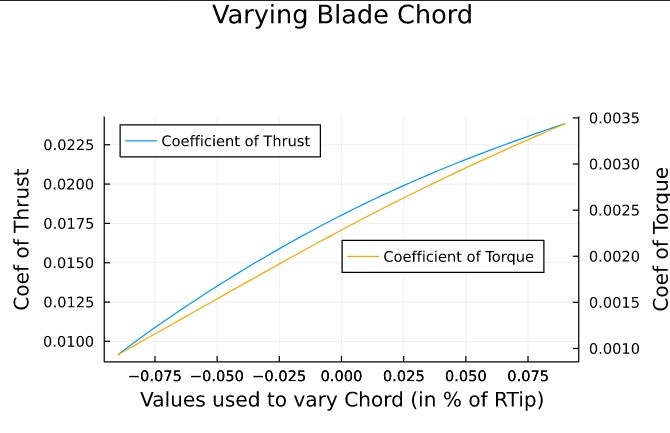
\includegraphics[scale = .75]{CVarCoefHMode.jpg}
\caption{The plot of the change in the coefficients of thrust (left y axis) and torque (right y axis) as the chord was increased. \textit{Note: In the geometry files the chord is given as a percent of the radius, so the chord variation was done by adding the shown chord percent to the chord value of each blade section of the standard blade. This means that at 0.05 the chord would be 6\% of Rtip if the original section was 1\% of Rtip for example.}}
\end{figure}

\textit{Coefficient of Thrust}\\
(See equation 1)\\
CT increases at a rate faster than $R^4$ and doesn't decrease (ie have a local max and then go down) at any point in the range, and although its' rate isn't increasing linearly it is very close. This shows that increasing the chord does not adversely affect CT similar to increasing the radius, however, unlike changing the radius, increasing the chord increases CT at a greater rate, and decreasing the chord is detrimental to CT (see Figure 5). Increasing chord does increase the amount of power and torque required.

\vspace{5mm} %5mm vertical space

\textit{Coefficients of Power and Torque}\\ 
(See equation 2)\\
CQ increases at a rate faster than $R^5$ and has behavior and trends similar to what was discussed in the CT section except that the increasing torque is generally not desired. This does highlight that decreasing the chord decreases the torque at a rate faster than decreasing radius does, a result that might at first seem intuitive. This behavior combined shows that varying chord is a very effective way to vary blade performance.

\vspace{5mm} %5mm vertical space

\begin{figure}[h]
\centering
\includegraphics[scale = .75]{CVarFMHmode.jpg}
\caption{The Figure of Merit as it varies with increasing chord.}
\end{figure}
\vspace{5mm} %5mm vertical space

\textit{Figure of Merit} \\
(See equation 3)\\
The figure of merit plot (Figure 6) shows that varying the chord has interesting affects. Decreasing the chord decreases performance, although much slower than decreasing pitch, and increasing the chord makes FM approach .76 which seems to be a possible limit/plateau. This maximum FM value is about the same max FM that varying the pitch was able to obtain. Varying chord obtains this max at about .05 (or a 5\% chord width increase) but is within 3\% of that value at the designers chosen chord width. Varying the chord should have a lower limit of about -.075 (or a 7.5\% chord width decrease) as by then it is just under 10\% less than its theoretical plateau/limit. It doesn't appear to need an upper limit, however it appears to have diminished returns and stop increasing, so an upper limit of .025 is probably sufficient as it is within 2\% of that theoretical max. There may be other design constraints that would restrict this range.

\vspace{5mm} %5mm vertical space


%%%%
\section{Findings from varying the Advance Ratio (J)}
The purpose of this section is to share the findings from varying the Advance Ratio the blade experiences and how it affects aerodynamic coefficients and their implications on blade performance. Derivations and explanations discussed above will not be re-discussed for the sake of brevity.

\vspace{5mm} %5mm vertical space

\begin{figure}[h]
\centering
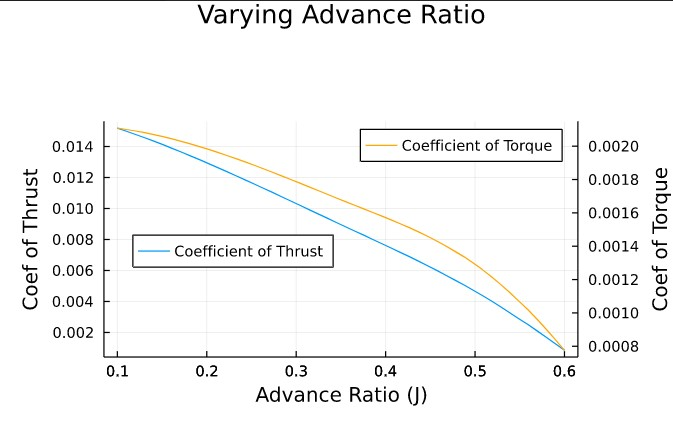
\includegraphics[scale = .75]{JVarCoefHMode.jpg}
\caption{The plot of the change in the coefficients of thrust (left y axis) and torque (right y axis) as the Advance Ratio was increased. \textit{Note: An Advance Ratio of 0 means that the blade (or drone/helicopter) is hovering and the rotor disc has no external inflow. A J of .8 means that the blade has an inflow that is .8 the rotational speed (ie experiencing a downdraft that fast, or flying upwards that fast, it can also be imagined as being thrown upwards)}}
\end{figure}

\textit{Coefficient of Thrust}\\
(See equation 1)\\
Increasing the Advance Ratio is only detrimental to CT as it causes it to decrease (See figure 7). It must be remembered however that without seeing the actual thrust numbers all that is known is that CT is increasing at a rate less than $R^4$ this means that mathematically it could be decreasing, or it could still be increasing, but just slower. However a quick glance at the Figure of Merit (figure 8) shows that regardless of what is happening to the actual thrust numbers blade performance goes down as J is increased. Thrust is generated (in its simplest form) by speeding up air and "throwing" it back. When that air is already sped up a little bit, less thrust is able to be generated. This is clearly seen in the CT plot, however not having to speed up the air as much leads to a decrease in power and torque required. Also note that increasing J by .1 (an inflow proportional to 10\% of the rotational speed) decreases CT from its original (with all things standard) .018 by 11\% and a J of .2 decreases it by 27\%, so it quickly a drastically affects performance.

\vspace{5mm} %5mm vertical space

\textit{Coefficients of Power and Torque}\\ 
(See equation 2)\\
CQ decreases as J increases as it is less difficult for the blade to "speed up" the air. This means that the amount of torque required is either decreasing or it is still increasing, but at a rate slower than $R^5$, as found in the discussion of the relationship above. Advance Ratios above .5 seem to have a greater effect on decreasing CQ, although any J above 0 has decreases CQ and thus CP also.

\vspace{5mm} %5mm vertical space

\begin{figure}[h]
\centering
\includegraphics[scale = .75]{JVarFMHmode.jpg}
\caption{The Figure of Merit as it varies with increasing Advance Ratios.}
\end{figure}
\vspace{5mm} %5mm vertical space

\textit{Figure of Merit} \\
(See equation 3)\\
The figure of merit plot (Figure 8) shows that increasing the Advance Ratio only decreases the figure of merit. This means that the power required to perform at the same level as J increases is higher than the ideal amount of power required. At a glance the relationship appears to be semi linear and the max FM occurs when J is 0 as expected. This means that even though CQ decreases as J increases, it doesn't matter as CT also decreases at a rate that makes the Figure of Merit also continuously decrease. All of the above seems to suggest that the designers (if using the blade at the chosen 5000 rpm) would have designed the blade for hover as its performance goes down quite quickly with the increasing Advance Ratios.

\vspace{5mm} %5mm vertical space

%%%%%
\section{Conclusion: Overall trends and implications, further research}
Overall it was found that varying the pitch and chord were the quickest and most effective ways to improve performance. Varying the blade radius can also improves performance, however it does so at a rate that under performs when compared to varying pitch and chord. As the pitch is varied performance increases as pitch is increased within certain limits, so the recommended range is between -3 and 8 degrees. Increasing the chord also increases performance, however also only within limits, so the recommended range is between -7.5\% and 2.5\%. Varying the blade radius does not have performance constraints, ie a certain radius doesn't provide an optimal CT value, it should be limited by constraints set by the designer however (minimum amounts of thrust required and maximum amounts of torque allowed etc). Increasing the Advance Ratio only decreases performance, however it seems to do so at a constant rate, so there are no recommended limits just a caution that advance ratio should be taken into consideration during the design process as a small change of J can quickly hurt blade performance.\\
The above recommended limits to the design space provide the designer with room to create a propeller that performs well at the tested 5000 RPM, however there does not seem to be an absolute "optimal" set of parameters. This means that there are inherent trade-offs between CT, CQ, and FM that will come depending on the designers goals and constraints and their chosen blade geometry.
The results of this trade study also highlighted that the chosen geometry and set of parameters that DJI chose performs quite well at 5000 RPM and would be good at hovering as it balances a decent CT with a slightly lower CQ, leading to a decent FM which in the real world would transfer to being able to hover with a decent sized load and still have quite good battery life. This is a common goal of drones especially the type of consumer camera drones that DJI specializes in.
More research will need to be done with varying RPMs and how that affects the blade performance, this was begun but is outside the scope of the paper, so surface plots showing coefficient results are only shown in the appendix. Research needs to be done with more Advance Ratios as well, especially with numbers that are realistic, not only for a drone climbing or descending, but also with forward flight and the effect of non perpendicular inflow to the blade disc.
\\
To offer advice, proffer questions, or voice concerns, please contact\\ Jacob Child: \href{mailto: childjacob2@gmail.com}{link}

\newpage
\section{\textbf{Appendix}}

\vspace{5mm} %5mm vertical space
\textit{Github Explanation}
This project can be found at \href{https://github.com/JacobChild/FlowLab_Onboarding/tree/main/TradeStudy}{Github Link}\\
The main file to run this study is TradeStudyTopFile.jl. It has been coded in such a way that if you set up your blade file structure (containing geometry and airfoil performance) in the same way as the "data" folder on my github. This data was found and copied from  \href{https://github.com/byuflowlab/FLOWUnsteady}{here} you only need to change the variable CmdFileName found around line 53 to your "command file" name. It should then be able to run and output all the analysis at 5000 RPM as well as give surface plots of varied rpm. Other parameters you may want to change are all found near the top of the file. Other files that are called by TradeStudyTopFile.jl are FunctionFile.jl this contains some necessary functions. The rest of the files (TSExtenderNSmootherFunction.jl, TSPolarPlotterFunction.jl) are used when the airfoil data is imported to extend and smooth it. They generate "CurrentAirfoilData.txt" that contains that data in the proper format for the TopFile to use. Each airfoil requires different smoothing values etc, but all of the necessary data/values are extracted from the "data" folder. If your geometry is not found in the data folder, you can generate new data using what is found under the "XFoilProject" folder found \href{https://github.com/JacobChild/FlowLab_Onboarding}{here}. The files are heavily commented and should be understandable.
The plots used in this paper are found under 5000RPM Outputs and Surface Outputs.

\vspace{5mm} %5mm vertical space
\textit{Surface plots} These show CT, CQ, and FM as functions of RPM and radius, pitch, chord and advance ratio\\
%\graphicspath{ {./surfaces/} }
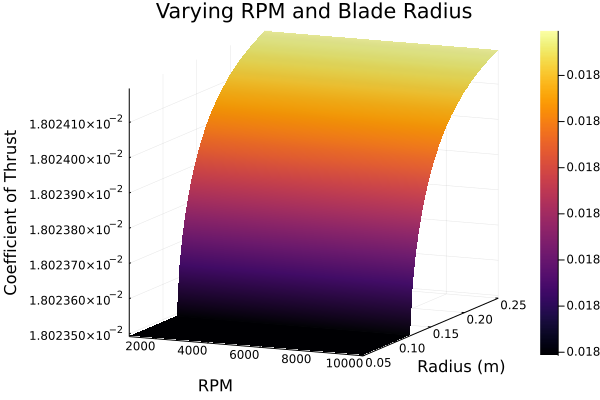
\includegraphics[scale=.65]{./surfaces/RVarCTSurfacePlot}\\
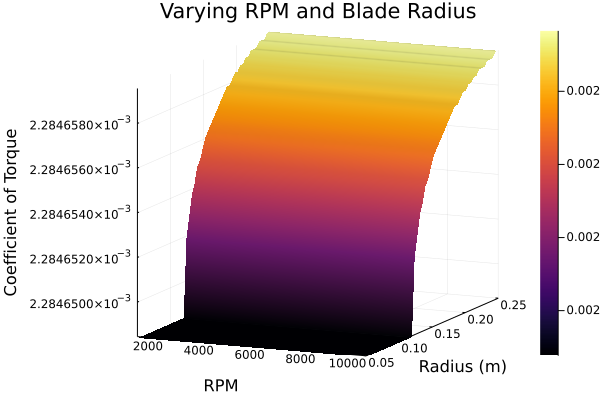
\includegraphics[scale=.65]{./surfaces/RVarCQSurfacePlot}\\
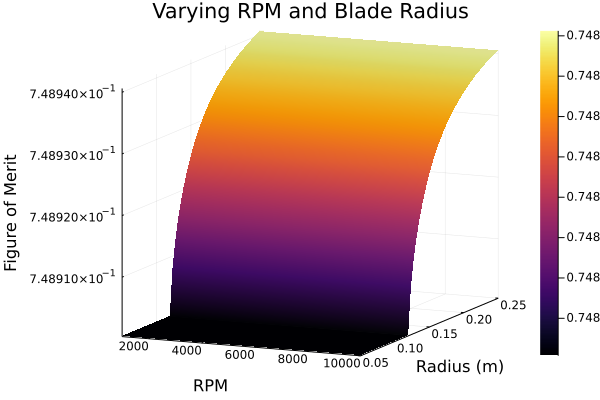
\includegraphics[scale=.65]{./surfaces/RVarFMSurfacePlot}\\
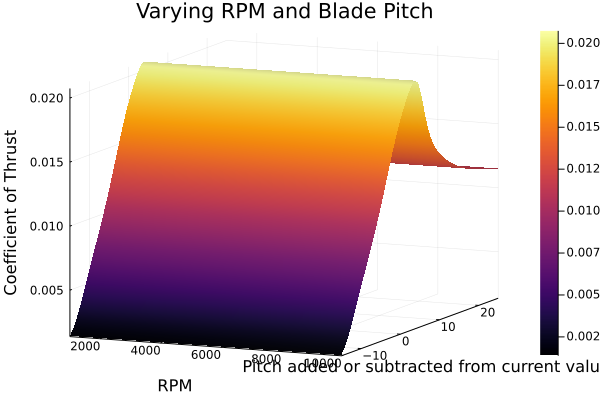
\includegraphics[scale=.65]{./surfaces/PVarCTSurfacePlot}\\
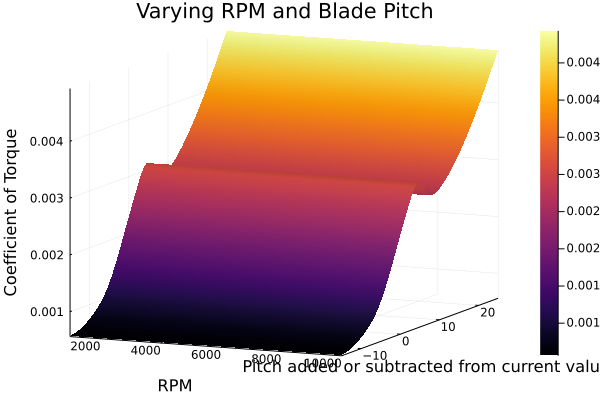
\includegraphics[scale=.65]{./surfaces/PVarCQSurfacePlot}\\
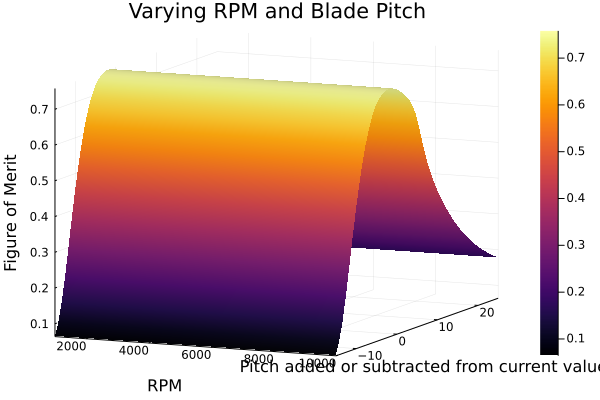
\includegraphics[scale=.65]{./surfaces/PVarFMSurfacePlot}\\
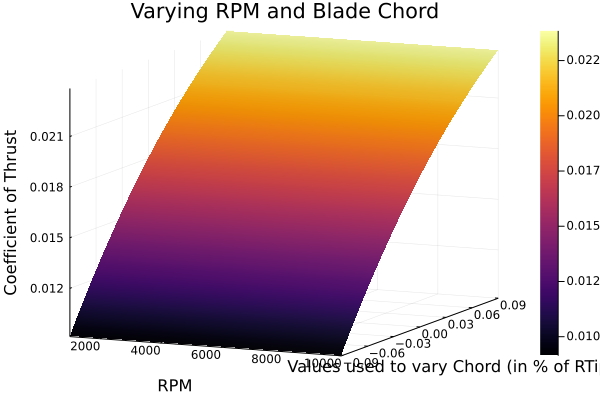
\includegraphics[scale=.65]{./surfaces/CVarCTSurfacePlot}\\
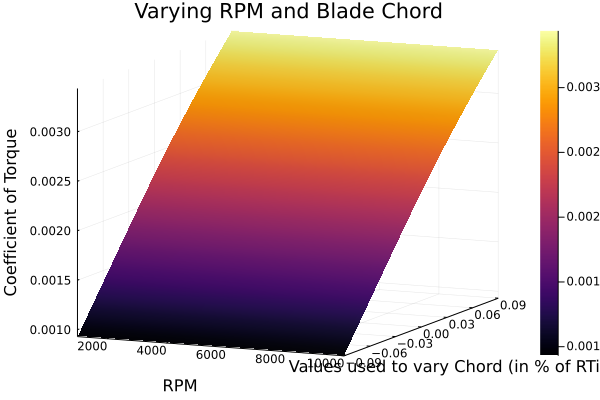
\includegraphics[scale=.65]{./surfaces/CVarCQSurfacePlot}\\
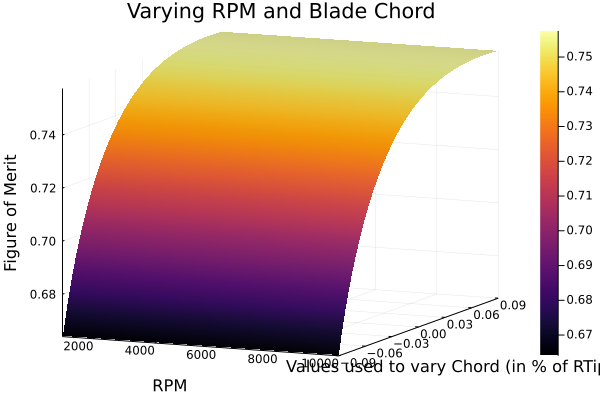
\includegraphics[scale=.65]{./surfaces/CVarFMSurfacePlot}\\
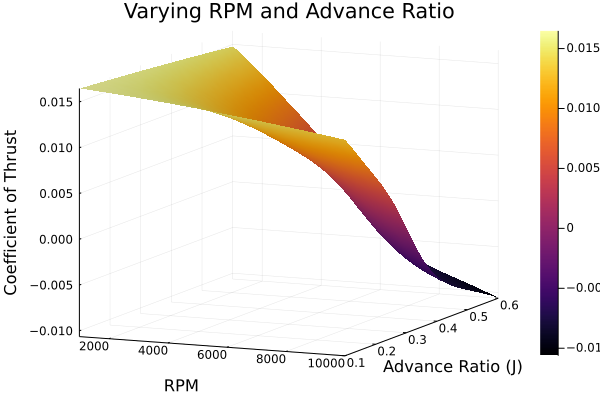
\includegraphics[scale=.65]{./surfaces/JVarCTSurfacePlot}\\
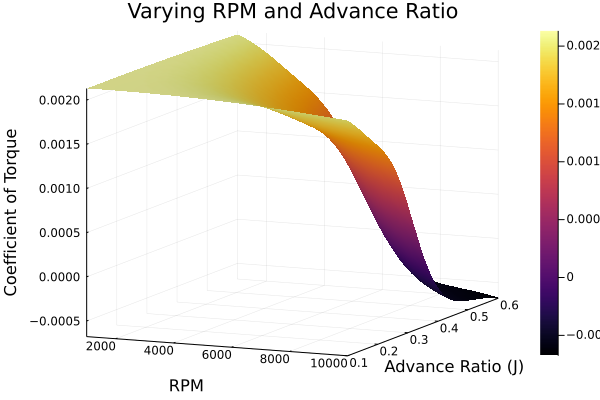
\includegraphics[scale=.65]{./surfaces/JVarCQSurfacePlot}\\
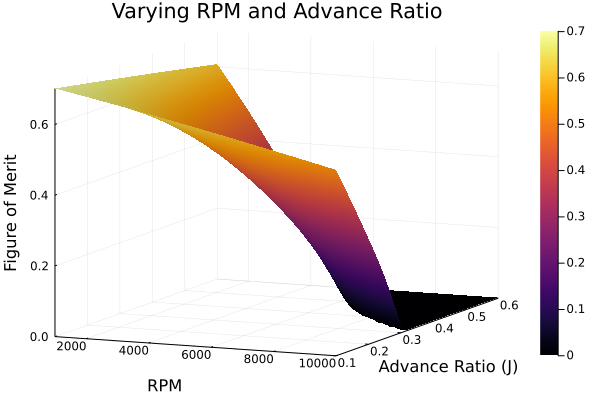
\includegraphics[scale=.65]{./surfaces/JVarFMSurfacePlot}\\


\end{document}